\documentclass{article}
\usepackage[utf8]{inputenc}
\usepackage[dvipsnames]{xcolor}
\usepackage{lmodern}
\usepackage{graphicx}
\usepackage{xcolor}
\graphicspath{ {./images/} }
\usepackage{imakeidx}
\makeindex[columns=3, title=Alphabetical Index, intoc]

\usepackage{tabularx}
\usepackage{paralist}


\usepackage[official]{eurosym}
\DeclareUnicodeCharacter{20AC}{\euro{}}

\author{Agosta, Belli, Emili, Giacchini, Luciani}



\begin{document}


\begin{center}
    \sffamily{\fontsize{50}{48} \selectfont \textcolor{red}{Nexi}\textcolor{green}{Fy}}
\end{center}

\begin{center}
    \itshape{\fontsize{20}{48} \selectfont streaming to your pocket}
\end{center}

\bigskip\bigskip\bigskip

\begin{flushleft}
    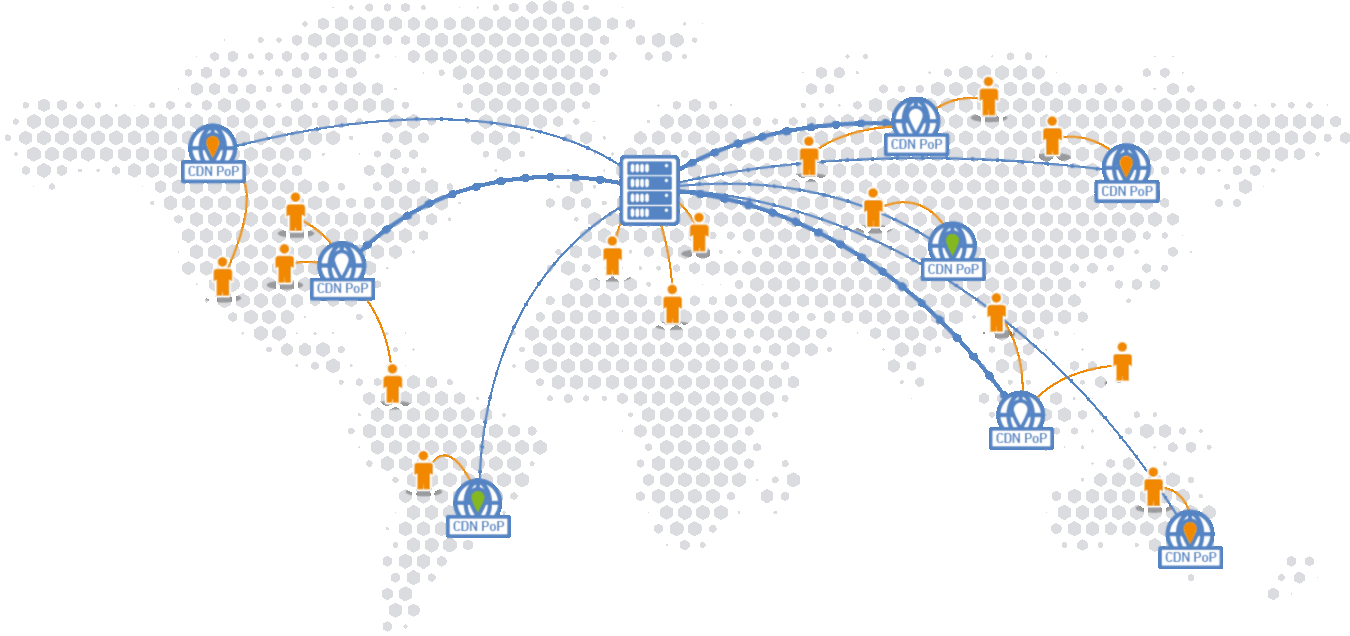
\includegraphics[scale=1]{images/worldCDN.png}
\end{flushleft}

\newpage
\printindex

\tableofcontents

\newpage
\section{\itshape{Glossario}}
 In questa sezione saranno esplicitati tutti i termini necessari alla comprensione del progetto.

\begin{itemize}
	%\item  \textbf{multimedia-manager}: servizio usato da partner per la gestione (caricamento/eliminazione) dei propri video e/o tracce audio. %viene citato solamente qui nel glossario
	\item \textbf{Piano di abbonamento}: pacchetto di funzionalità, acquistabile dagli utenti per un certo periodo (e rinnovabile alla fine del periodo). A volte è indicato impropriamente come "abbonamento"
	\item \textbf{API}: interfaccia offerta all'esterno di un sistema, per poter usare delle funzionalità interne al sistema
	\item \textbf{CDN}: sistema di server largamente distribuita, usata per la distribuzione di contenuti quali tracce video e audio.
	\item \textbf{ORM}: tecnica per interfacciarsi con basi di dati relazionali, astraendo dall'implementazione del dbms
	\item \textbf{Piattaforma}: componente del sistema accessibile dagli utenti.
	\item \textbf{Server}: macchina logica (composta da uno o piu macchine fisiche) su cui risiede la piattaforma in parte o nella sua totalità.
	\item \textbf{RUP}: Rational Unified Process, processo di sviluppo basato su fasi temporali, iterazioni e attività.
	\item \textbf{Risorsa Multimediale}: intendiamo un file di tipo multimediale, quindi un video, una canzone, ecc. (a volte è indicata solamente come risorsa)
	\item \textbf{Prodotto}: si intende un singolo prodotto video o audio creato da un partner (e.g: un singolo film, una singola canzone, un singolo episodio di una serie tv, ecc.)
	\item \textbf{Playlist}: lista ordinata di prodotti
	\item \textbf{Contenuto}: un singolo prodotto o una playlist
\end{itemize}
\index{Index}

\newpage
\section{\itshape{Visione del Sistema}}
\textbf{NexiFy} è una piattaforma di streaming multimediale on demand che offre contenuti quali film, serie tv, brani e video musicali e altre forme di intrattenimento. Il servizio è fruibile sia via web che da app mobile.\\

La fruizione dei contenuti avviene attraverso un singolo player audio / video:
\begin{itemize}\item per la riproduzione di film o serie tv entrambe le tracce video e audio vengono riprodotte in contemporanea. L’utente può scegliere la qualità di riproduzione, manualmente o automaticamente, in base alle sue preferenze e disponibilità di connessione a internet. Possono essere mostrati anche dei sottotitoli (se disponibili).
    \item per la riproduzione di musica ci sono due scenari diversi (in entrambi i casi il brano può essere ascoltato con l’app in background, inibendo quindi la traccia video) :
    \begin{enumerate}
        \item il brano è accompagnato dal relativo video musicale; in questo caso vengono riprodotte entrambe le tracce audio e video contemporaneamente.
        \item il brano non è accompagnato dal video musicale; in questo caso viene riprodotta la sola traccia audio e al posto della traccia video, viene mostrata la copertina dell’album relativo al brano oppure i lyrics del brano in tempo reale (in base alla scelta dell’utente e alla disponibilità dei lyrics).
    \end{enumerate}
\end{itemize}
    
Gli utenti della piattaforma si dividono in due categorie: partner e iscritti.\\

I contenuti sono caricati da partner che sottoscrivono un contratto di collaborazione, pagando una quota annuale uguale per tutti ma modificabile nel corso del tempo. Questi ultimi ricevono un compenso in base al numero di riproduzioni che hanno ottenuto sui loro contenuti.\\

Gli iscritti sono coloro che usufruiscono del servizio; essi hanno la possibilità di scegliere diversi profili di abbonamento definibili a piacere tramite apposite funzioni di creazione a associazione degli abbonamenti alle varie funzionalità offerte dal sistema.\\

Questo servizio dà la possibilità agli iscritti interessati di visualizzare film e serie tv e ascoltare brani musicali sottoscrivendo un singolo abbonamento. Questo porta ad essi un risparmio di denaro, in quanto non è necessario iscriversi a diversi servizi il cui costo totale ammonterebbe ad una quota mensile maggiore.\\

\subsection{\itshape{Vincoli}}
NexiFy si riserva la possibilità di rimuovere qualsiasi contenuto video e/o audio presente sulla piattaforma che, dopo previa verifica, non rispetta la linee guida dei TOS.
In particolare è vietato il caricamento di qualsiasi traccia audio/video con contenuti sessualmente espliciti o che promuovono o giustificano l'uso della violenza contro persone o gruppi in base a razza, etnia, religione, disabilità fisiche, sesso, età, nazionalità né contenuti il cui scopo sia l'incitamento all'odio sulla base di tali caratteristiche.

\index{Index}

\newpage
\section{\itshape{Configurazione del Sistema alla Consegna}}
Alla consegna del sistema prevediamo, già inclusi in esso, i seguenti abbonamenti designati e pensati per gli utenti:
\begin{itemize}
    \item Free (0 € / mese ) che darà accesso alle seguenti funzioni: 
	\begin{itemize}
   		\item Ascoltare brani musicali presenti sulla piattaforma \textbf{con} limiti di scelta di riproduzione e intermezzi pubblicitari;
		\item Visionare episodi pilota di serie tv;
		\item Visionare trailer di film.
	\end{itemize}
    \item Music (9.99 € / mese) che darà accesso alle seguenti funzioni:
	\begin{itemize}
   		\item Ascoltare brani musicali presenti sulla piattaforma \textbf{senza} limiti di scelta di riproduzione e intermezzi pubblicitari;
		\item Scaricare su dispositivo, tramite app mobile, brani musicali per usufruirne offline;
		\item Visionare episodi pilota di serie tv;
		\item Visionare trailer di film.
	\end{itemize}
    \item Premium (14.99 € / mese) che darà accesso alle seguenti funzioni:
	\begin{itemize}
   		\item Ascoltare brani musicali presenti sulla piattaforma \textbf{senza} limiti di scelta di riproduzione e intermezzi pubblicitari;
		\item Scaricare su dispositivo, tramite app mobile, brani musicali per usufruirne offline;
		\item Visionare tutti gli episodi delle serie tv presenti sulla piattaforma;
		\item Scaricare su dispositivo, tramite app mobile, episodi di serie tv per usufruirne offline;
		\item Visionare tutti i film presenti sulla piattaforma.
		\item Scaricare su dispositivo, tramite app mobile, film per usufruirne offline;
	\end{itemize}
	
	\item Partner (300 € / anno) che darà accesso alle seguenti funzioni:
	\begin{itemize}
   		\item Pubblicazione di video
		\item Pubblicazione di brani musicali
		\item Modifica/rimozione di video
		\item Modifica/rimozione di brani musicali
		\item Ricevere pagamenti in base alle visualizzazioni sui propri contenuti
	\end{itemize}
\end{itemize}


La CDN fornita coprirà l’intera area geografica globale arrivando in tempi ragionevoli a tutti gli utenti. Inoltre supporterà un numero massimo di XXXX utenti.


\index{Index}

\newpage
\section{\itshape{Studio di Fattibilità}}
\subsection{Aspetto tecnologico}
Per la realizzazione del sistema sarà necessario l'utilizzo di CDN, in modo da distribuire i contenuti multimediali in maniera efficiente e mantenendoli sempre accessibili per gli utenti. Deve inoltre essere possibile, in maniera efficiente, estrarre dati e statistiche dalla CDN (come per esempio quante volte è stato richiesto un certo video in una certa zona). Saranno necessarie basi di dati relazionali cloud-based per mantenere informazioni su dati utenti (oltre alle informazioni di base, anche le eventuali playlist musicali create, ecc), e implementando funzionalità lato server per gestire le richieste degli utenti, la loro autenticazione e altro. Verrà inoltre utilizzato un ORM per garantire semplicità di migrazione ad un'altra tecnologia di memorizzazione dati permettendo di rendere indipendente il codice dalla base di dati.\\
La fattibilità del progetto dal punto di vista tecnologico segue dalla grande disponibilità di aziende che offrono servizi cloud, tra cui CDN: per esempio AWS CloudFront. Questi servizi includono anche delle API per interfacciarsi in maniera efficiente con la CDN. Notiamo che questi servizi vengono già usati da piattaforme simili a NexiFy, e che sono risultate in grado di scalare a livello mondiale (ad esempio Prime Video usa AWS CloudFront). Anche per quanto riguarda i database esistono numerose soluzioni cloud affidabili.
%Il mantenimento dei dati riguardanti gli utenti sarà conforme alle politiche GDPR per garantire la privacy secondo le leggi europee.\\


%Per la realizzazione della piattaforma sarà necessario l’utilizzo di CDN per distribuire sul territorio contenuti multimediali mantenendo questi ultimi sempre accessibili in maniera ottimale da qualsiasi posizione geografica. Deve inoltre essere possibile, in maniera efficiente, estrarre dati e statistiche sugli accessi alla CDN. Si useranno basi di dati relazionali cloud-based per mantenere informazioni su dati utenti, e implementando funzionalità lato server per gestire le richieste degli utenti, la loro autenticazione e altro.Verrà inoltre utilizzato un ORM per garantire semplicità di migrazione ad un'altra tecnologia di memorizzazione dati permettendo di rendere indipendente il codice dalla base di dati.

\subsection{Aspetto Economico}
\subsubsection{Vantaggi del sistema}

NexiFy sarà in grado di acquisire utenti grazie ai diversi vantaggi offerti:
    \begin{itemize}
        \item La disponibilità di contenuti sia video che musicali, non presente in piattaforme quali Netflix e Spotify. Questo darà la possibilità agli utenti interessati di visualizzare film, serie tv e ascoltare brani musicali sottoscrivendo un singolo abbonamento, comportando un risparmio di denaro, in quanto non è necessario iscriversi a diversi servizi il cui costo totale ammonterebbe ad una quota mensile maggiore;
        \item La possibilità per piccoli creatori di pubblicare autonomamente contenuti, ma senza degradare la qualità dei contenuti (come invece avviene in piattaforme quali YouTube).

\subsubsection{Stima dei costi}
NexiFy inizialmente supporterà un numero modesto di utenti e di contenuti multimediali; questo per avere dei costi iniziali sostenibili, e man mano che si acquisiranno utenti (e quindi sottoscrizioni di abbonamenti) sarà possibile ampliare la CDN e i database (dal punto di vista software NexiFy sarà già progettato per supportare un carico maggiore del carico iniziale).

\textbf{todo... conti precisi}

    \end{itemize}
\index{Index}

\newpage
\section{\itshape{Vincoli}}
\begin{itemize}
\item NexiFy si riserva di modificare la quota annuale per i partner.
\item NexiFy si riserva di rimuovere ogni contenuto considerato non idoneo ad essere visualizzato o riprodotto dagli utenti.
\item In caso di contenuti particolari, prima della riproduzione l'utente verrà informato, dando la possibilità di evitare contenuti non desiderati.
\item In particolare è vietato il caricamento di qualsiasi traccia audio/video con contenuti sessualmente espliciti o che promuovono o giustificano l'uso della violenza contro persone o gruppi in base a razza, etnia, religione, disabilità fisiche, sesso, età, nazionalità né contenuti il cui scopo sia l'incitamento all'odio sulla base di tali caratteristiche. 
\item NexiFy può creare/modificare/rimuovere profili di abbonamento. 
\item Qualsiasi risorsa audio o video scaricata tramite l'app mobile sarà codificata in modo tale da rendere il file accessibile \textbf{solo ed esclusivamente} tramite il player dell'app stessa onde evitare una riproduzione non consentita di questi.
\end{itemize}
 


\index{Index}

\newpage
\section{\itshape{Contratto}}
Il sistema che si intende realizzare viene descritto ad alto livello nella sezione 2 "Visione del sistema".\\
Le specifiche dettagliate del sistema si troveranno più avanti nel documento.\\
Nella sezione 3 "Studio della fattibilità" si possono trovare le motivazioni che rendono possibile affermare che
il sistema è realizzabile e la stima dei costi che la realizzazione stessa comporterà.\\
Il team si impegnerà a realizzare il sistema in questione in un periodo non maggiore di 5 mesi.\\
Questo contratto non può essere ceduto, in tutto o in parte, a terzi rispetto a coloro che hanno firmato lo stesso, ad esclusione del caso in cui venga ottenuta una specifica autorizzazione.


\subsection{Descrizione del Sistema}

\subsubsection{Introduzione}
In questa sezione verrà fatta una descrizione del sistema che scende in maggiori dettagli rispetto a quanto
si è fatto in precedenza nel documento.

\subsubsection{Interazione con gli utenti}
La piattaforma è indirizzata principalmente alla fruzione di contenuti, quali brani musicali, film e serie tv.\\
Al momento della consegna iniziale, i contenuti potranno essere visionati attraverso web app e app per mobile.
La web app è pensata per l'uso in casa, in quanto da la possibilità di visualizzare film e serie tv su schermi
di diverse dimensioni ed è accessibile anche da smart tv. L'app per mobile, invece, è pensata per una
interazione in mobilità, offrendo un'interfaccia più versatile e la possibilità di riprodurre brani musicali
quando l'app si trova in modalità background nel sistema operativo mobile.\\
Per quanto rigurda il player, esso viene descritto in dettaglio nella "Visione del Sistema".\\
Sulla piattaforma saranno inizialmente presenti dei listing dei contenuti che sono stati caricati, organizzati per 
categoria e tipo di risorsa multimediale (es. brano musicale o video). I contenuti potranno essere trovati
con una ricerca per titolo, autore, ecc.. Inoltre, agli utenti saranno suggerite delle nuove uscite,
oppure altri elementi che potrebbero interessargli.\\

\subsubsection{Accesso alla piattaforma}
Gli utenti che vorranno usufruire dei servizi offerti, dovranno sottoscrivere un abbonamento. Esisteranno diversi
tipi di abbonamento che saranno svincolati dagli insiemi di servizi a cui danno accesso. Quindi, una volta definiti
i servizi, gli amministratori della piattaforma potranno modellare degli abbonamenti che includono alcuni o
tutti questi servizi. Di conseguenza, i tipi di abbonamento offerti alla consegna potranno non essere più
disponibili dopo del tempo e potranno esserne costruiti di nuovi.
Le prime offerte sono descritte nella "Configurazione del Sistema alla Consegna".

\subsubsection{Pubblicazione dei contenuti}
NexiFy dà la possibilità a chiunque, in seguito alla sottoscrizione di un contratto da Partner,
di caricare contenuti sulla piattaforma. In questo modo viene permesso ai creatori amatoriali o emergenti,
di pubblicare i loro lavori, senza doversi necessariamente affidare a case produttrici od aver a disposizione
un grande budget.\\
Al momento della pubblicazione, verrà richiesto al Partner di inserire delle informazioni riguardanti
il contenuto proposto. Tra queste vi sono:
\begin{itemize}
    \item Titolo 
    \item Descrizione breve
    \item Descrizione completa
    \item Tipo (es. film o brano musicale)
    \item Categoria
    \item Collezione, se applicabile
    \item Pubblico consigliato
\end{itemize}
In alcuni casi, i singoli elementi caricati verranno organizzati in collezioni. Ad esempio, gli espisodi delle
serie TV appartengono alle serie stesse, oppure, i brani musicali appartengono ad album.\\
Alcuni contenuti potrebbero non essere indicati per un pubblico giovanile, quindi il Partner dovrà rispondere ad
un questionario che lo aiuterà a classificare la sua pubblicazione e a generare delle opportune etichette
relative alle fasce d'età consentite. Nel caso in cui un Partner dichiarasse il falso nei questionari, ci 
saranno ripercussioni più o meno gravi sul suo account che possono arrivare fino alla sospensione definitiva
di quest'ultimo.

\index{Index}

\newpage
\section{\itshape{Descrizione del Sistema}}


\index{Index}

\newpage
\section{\itshape{Pianificazione del Progetto}}
\setlength{\arrayrulewidth}{.5mm}
\setlength{\tabcolsep}{5pt}
\renewcommand{\arraystretch}{2}

\subsection{Introduzione}
Il team seguirà la metodologia di progetto RUP, in seguito sono specificati il piano di progetto e le
iterazioni che lo compongono.

\subsection{Piano}
Il piano di progetto si suddivide in 4 fasi temporali:
\begin{itemize}
    \item Inception
    \item Elaboration
    \item Construction
    \item Transition
\end{itemize}
Le attività coinvolte sono le seguenti:
\begin{itemize}
    \item Studio di fattibilità
    \item Raccolta dei requisiti
    \item Analisi e progetto
    \item Implementazione
    \item Test
\end{itemize}
Le varie attività si distribuiranno nelle fasi temporali in maniera eterogenea, in relazione a quanto una particolare attività è significativa in una certa fase. Qui sotto è raffigurato il processo in un grafico descrittivo: \vspace{0.6cm}

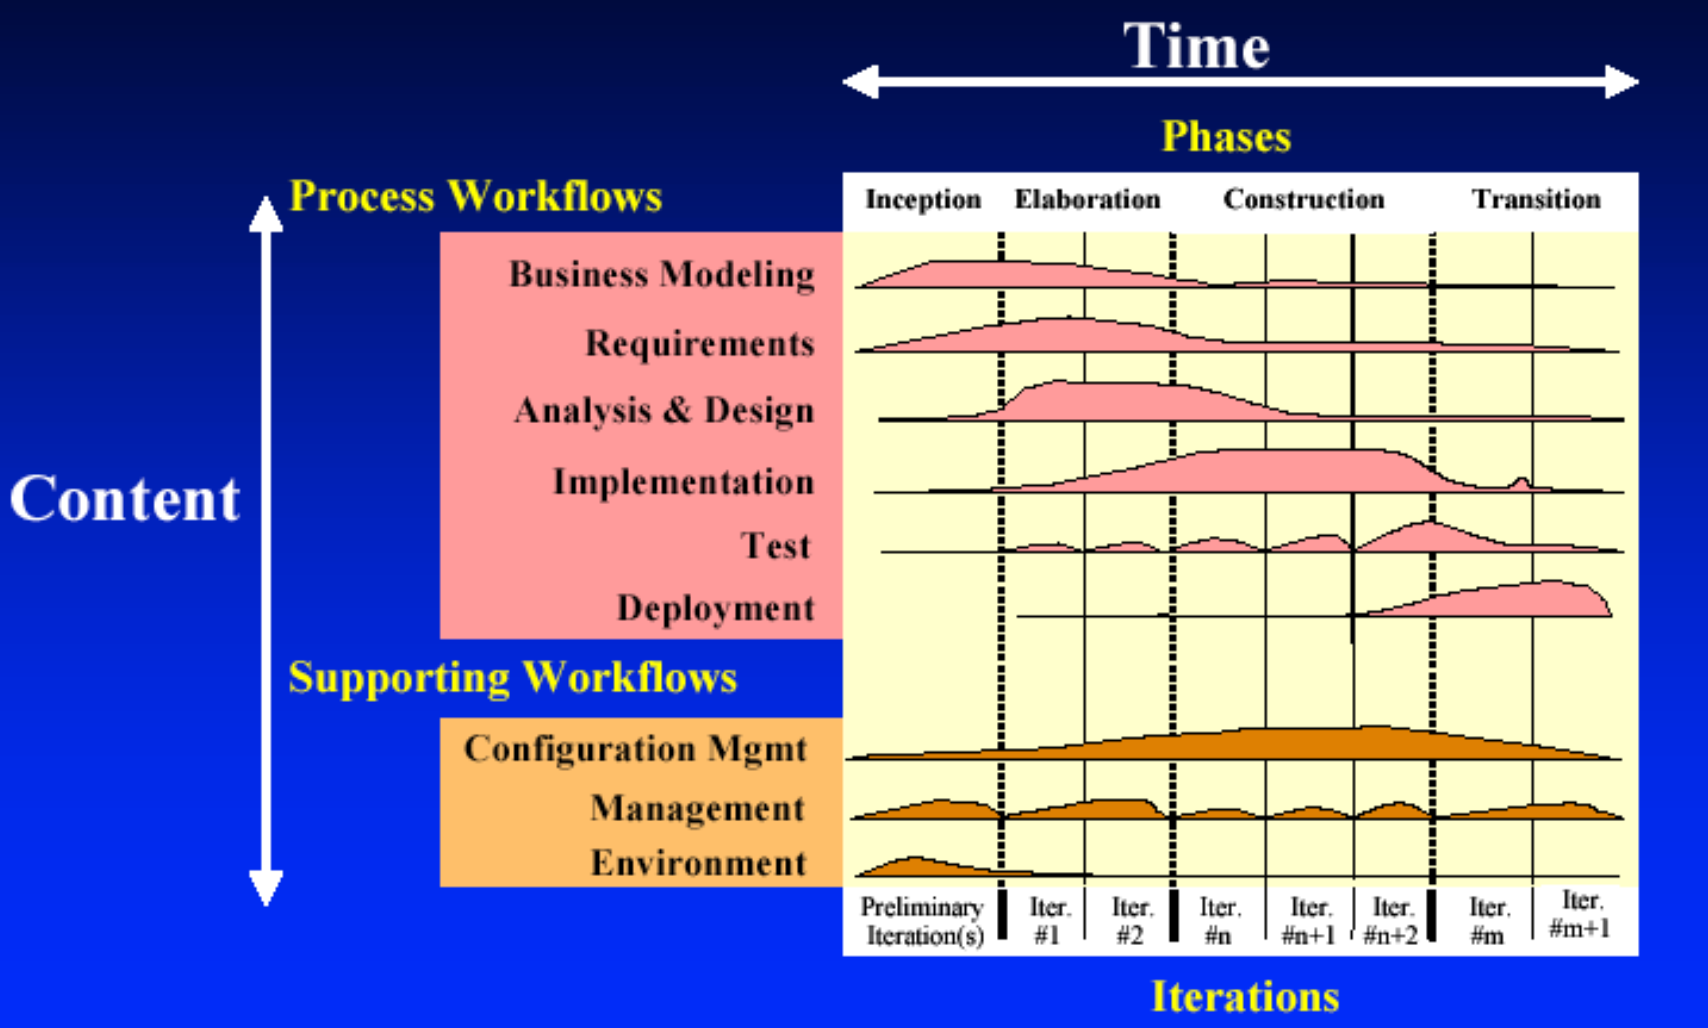
\includegraphics[width=12cm]{RUPplan.png}

\subsection{Iterazioni}

\emph{\textbf{Nota:}} si assume che i requisiti funzionali primari sono tutti quei requisiti con priorità alta e che potrebbero impattare sull'architettura. Al contrario, i requisiti funzionali secondari sono tutti i requisiti con priorità piu bassa e che non hanno impatto sull'architettura.

\begin{center}

\begin{tabular}{ |p{2cm}|p{10cm}|  }
\hline
Nome & Iterazione 1 \\\hline
Fase & Inception \\\hline
Inizio & 20/11/2019 \\\hline
Fine &  1/12/2019 \\\hline
Obbiettivi & 
	\begin{compactitem}
		\item Analisi del problema e prima stesura del documento di Visione
		\item Definire configurazione iniziale del sistema
		\item Analizzare la fattibilità del progetto, dal punto di vista tecnico ed economico
		\item Formulazione di una prima proposta di Contratto
		\item Formulazione documento Glossario
	\end{compactitem}\\\hline
Stato &  Conclusa \\\hline
\end{tabular}
\label{table:1}\newline

\begin{tabular}{ |p{2cm}|p{10cm}|  }
\hline
Nome & Iterazione 2 \\\hline
Fase & Inception \\\hline
Inizio & 15/12/2019 \\\hline
Fine &  18/12/2019 \\\hline
Obbiettivi & 
	\begin{compactitem}
		\item Stesura del piano di progetto
		\item Revisione e aggiornamento della proposta di contratto
		\item Individuare almeno il 50\% dei requisiti funzionali con priorità primaria
	\end{compactitem}\\\hline
Stato &  Conclusa \\\hline
\end{tabular}
\label{table:2}\newline

\begin{tabular}{ |p{2cm}|p{10cm}|  }
\hline
Nome & Iterazione 3 \\\hline
Fase & Inception \\\hline
Inizio & 01/02/2020 \\\hline
Fine &  14/02/2020 \\\hline
Obbiettivi & 
	\begin{compactitem}
		\item Individuare tutti i rimanenti requisiti funzionali con priorità primaria
		\item Individuare almeno il 25\% dei requisiti non funzionali
		\item Descrivere ad alto livello i requisiti individuati
		\item Individuare almeno il 70\% dei rischi e stendere un piano di gestione per ciascun rischio
	\end{compactitem}\\\hline
Stato &  Conclusa \\\hline % Svolgimento 
\end{tabular}
\label{table:3}\newline

\begin{tabular}{ |p{2cm}|p{10cm}|  }
\hline
Nome & Milestone 1\\\hline
Fase & Inception \\\hline
Inizio & 17/02/2020 \\\hline
Fine &  17/02/2020 \\\hline
Obbiettivi & 
	\begin{compactitem}
		\item I requisiti funzionali primari sono stati individuati e descritti correttamente
		\item Almeno il 70\% dei rischi è stato individuato ed è stato creato un piano di gestione per ciascun rischio
		\item Tutte le iterazioni sono state programmate
	\end{compactitem}\\\hline
Stato &  Raggiunta \\\hline
\end{tabular}
\label{table:milestone1}\newline

\begin{tabular}{ |p{2cm}|p{10cm}|  }
\hline
Nome & Iterazione 4 \\\hline
Fase & Elaboration \\\hline
Inizio & 17/02/2020 \\\hline
Fine &  24/02/2020 \\\hline
Obbiettivi & 
	\begin{compactitem}
		\item Iniziare modello di analisi dell'architettura, individuando le classi
		\item Definire il modello dei casi d'uso per il primo 50\% dei requisiti funzionali primari
		\item Individuare 5 requisiti funzionali fondamentali tra i requisiti funzionali primari (che verranno usati per testare l'architettura)
		\item Individuare e descrivere un ulteriore 50\% dei requisiti non funzionali
		\item Individuare un ulteriore 15\% dei rischi e stendere un piano di gestione per ciascun rischio
	\end{compactitem}\\\hline
Stato &  Conclusa \\\hline
\end{tabular}
\label{table:4}\newline

\begin{tabular}{ |p{2cm}|p{10cm}|  }
\hline
Nome & Iterazione 5 \\\hline
Fase & Elaboration \\\hline
Inizio & 26/02/2020 \\\hline
Fine &  03/03/2020  \\\hline
Obbiettivi & 
	\begin{compactitem}
		\item Completare il modello di analisi dell'architettura (completare la descrizione delle classi ed effettuare una suddivisione in package)
		\item Completare il modello dei casi d'uso relativo ai requisiti funzionali primari
		\item Individuare e descrivere i restanti requisiti non funzionali % 100%
		\item Individuare i rischi rimanenti e stendere un piano di gestione per ciascun rischio % 100%
		\item Individuare i primi test sull'architettura e sui requisiti fondamentali
		\item Effettuare una stima dei costi con casi d'uso primari
	\end{compactitem}\\\hline
Stato &  Conclusa \\\hline
\end{tabular}
\label{table:5}\newline

\begin{tabular}{ |p{2cm}|p{10cm}|  }
\hline
Nome & Iterazione 6 \\\hline
Fase & Elaboration \\\hline
Inizio & 05/03/2020 \\\hline
Fine &  14/03/2020  \\\hline
Obbiettivi & 
	\begin{compactitem}		
		\item Iniziare il modello di design dell'architettura
		\item Definire il modello di analisi per i casi d'uso fondamentali individuati
		\item Ampliare i test sull'architettura e sui requisiti fondamentali, in seguito alle scelte di progetto		

	\end{compactitem}\\\hline
Stato &  Programmata \\\hline
\end{tabular}
\label{table:6}\newline

\begin{tabular}{ |p{2cm}|p{10cm}|  }
\hline
Nome & Iterazione 7 \\\hline
Fase & Elaboration \\\hline
Inizio & 15/03/2020 \\\hline
Fine & 25/03/2020 \\\hline
Obbiettivi & 
	\begin{compactitem}
		\item Completare il modello di design dell'architettura
		\item Definire il modello di design per i casi d'uso fondamentali individuati
		\item Implementare l'architettura e i casi d'uso fondamentali individuati
		\item Ultimare i test sull'architettura e sui requisiti fondamentali
	\end{compactitem}\\\hline
Stato &  Programmata \\\hline
\end{tabular}
\label{table:7}\newline

\begin{tabular}{ |p{2cm}|p{10cm}|  }
\hline
Nome & Milestone 2\\\hline
Fase & Elaboration \\\hline
Inizio & 26/03/2020 \\\hline
Fine &  26/03/2020 \\\hline
Obbiettivi & 
	\begin{compactitem}
		\item Tutti i rischi sono stati individuati ed è stato creato un piano di gestione per ciascun rischio
		\item \'E stata effettuata una stima dei costi attendibile
		\item Prendere una decisione Go/NoGo
		\item \'E stata creata una base architetturale coerente con i requisiti ed eseguibile
		\item \'E stato prodotto un modello dei casi d'uso primari sufficientemente dettagliato per iniziare la fase di construction
		\item I casi d'uso fondamentali risultano implementati correttamente con l'architettura prodotta
	\end{compactitem}\\\hline
Stato &  Programmata \\\hline
\end{tabular}
\label{table:milestone2}\newline

\begin{tabular}{ |p{2cm}|p{10cm}|  }
\hline
Nome & Iterazione 8 \\\hline
Fase & Construction \\\hline
Inizio & 27/03/2020 \\\hline
Fine &  04/04/2020  \\\hline
Obbiettivi & 
	\begin{compactitem}

		\item Definire il modello di analisi per il 30\% dei requisiti funzionali primari
		\item Definire il modello di design per il 30\% dei requisiti funzionali primari
		\item Implemetazione e definizione dei test per il 30\% dei requisiti funzionali primari
	\end{compactitem}\\\hline
Stato &  Programmata \\\hline
\end{tabular}
\label{table:8}\newline

\begin{tabular}{ |p{2cm}|p{10cm}|  }
\hline
Nome & Iterazione 9 \\\hline
Fase & Construction \\\hline
Inizio & 05/04/2020 \\\hline
Fine &  12/04/2020  \\\hline
Obbiettivi & 
	\begin{compactitem}
		\item Definire il modello di analisi per un altro 30\% dei requisiti funzionali primari
		\item Definire il modello di design per un altro 30\% dei requisiti funzionali primari
		\item Implementazione e definizione dei test per il 30\% dei requisiti funzionali primari
		
	\end{compactitem}\\\hline
Stato &  Programmata \\\hline
\end{tabular}
\label{table:9}\newline


\begin{tabular}{ |p{2cm}|p{10cm}|  }
\hline
Nome & Iterazione 10 \\\hline
Fase & Construction \\\hline
Inizio & 13/04/2020 \\\hline
Fine &  20/04/2020  \\\hline
Obbiettivi & 
	\begin{compactitem}
		\item Definire il modello di analisi per un altro 30\% dei requisiti funzionali primari
		\item Definire il modello di design per un altro 30\% dei requisiti funzionali primari
		\item Implementazione e definizione dei test per il 30\% dei requisiti funzionali primari
		
		\item individuazione e definizione del modello dei casi d'uso per i requisiti funzionali secondari
	\end{compactitem}\\\hline
Stato &  Programmata \\\hline
\end{tabular}
\label{table:10}\newline

\begin{tabular}{ |p{2cm}|p{10cm}|  }
\hline
Nome & Iterazione 11 \\\hline
Fase & Construction \\\hline
Inizio & 21/04/2020 \\\hline
Fine &  27/04/2020  \\\hline
Obbiettivi & 
	\begin{compactitem}
		\item Definire il modello di analisi per il restante 10\% dei requisiti funzionali primari
		\item Definire il modello di design per il restante 10\% dei requisiti funzionali primari
		\item Implementazione e definizione dei test per il 10\% dei requisiti funzionali primari
		
		\item Definire il modello di analisi dei requisiti funzionali secondari
		\item Definire il modello di design per dei requisiti funzionali secondari
		\item Implementazione e definizione dei test dei requisiti funzionali secondari
		
	\end{compactitem}\\\hline
Stato &  Programmata \\\hline
\end{tabular}
\label{table:11}\newline


\begin{tabular}{ |p{2cm}|p{10cm}|  }
\hline
Nome & Milestone 3\\\hline
Fase & Construction \\\hline
Inizio & 28/04/2020 \\\hline
Fine &  28/04/2020 \\\hline
Obbiettivi & 
	\begin{compactitem}
		\item Sono stati definiti test per ogni funzionalità del sistema
		\item Il sistema e le sue funzionalità implementate hanno superato tutti i test definiti
	\end{compactitem}\\\hline
Stato &  Programmata \\\hline
\end{tabular}
\label{table:milestone3}\newline

\begin{tabular}{ |p{2cm}|p{10cm}|  }
\hline
Nome & Iterazione 12 \\\hline
Fase & Transition \\\hline
Inizio & 29/04/2020 \\\hline
Fine &  2/05/2020  \\\hline
Obbiettivi & 
	\begin{compactitem}
		\item Raccolta Feedback di utilizzo degli utenti
		\item Effettuare correzioni basate sul feedback degli utenti
		\item Creazione degli ultimi test basati sul feedback degli utenti
		\item Creare una release finale
	\end{compactitem}\\\hline
Stato &  Programmata \\\hline
\end{tabular}
\label{table:12}\newline

\begin{tabular}{ |p{2cm}|p{10cm}|  }
\hline
Nome & Milestone 4\\\hline
Fase & Transition \\\hline
Inizio & 03/05/2020 \\\hline
Fine &  03/05/2020 \\\hline
Obbiettivi & 
	\begin{compactitem}
		\item Release finale creata
		\item La release finale supera i test definiti in seguito al feedback degli utenti
	\end{compactitem}\\\hline
Stato &  Programmata \\\hline
\end{tabular}
\label{table:milestone4}\newline


\end{center}

\subsection{Diagramma di Gantt}
\vspace{0.5cm}
\begin{center}
	\hspace*{-2cm}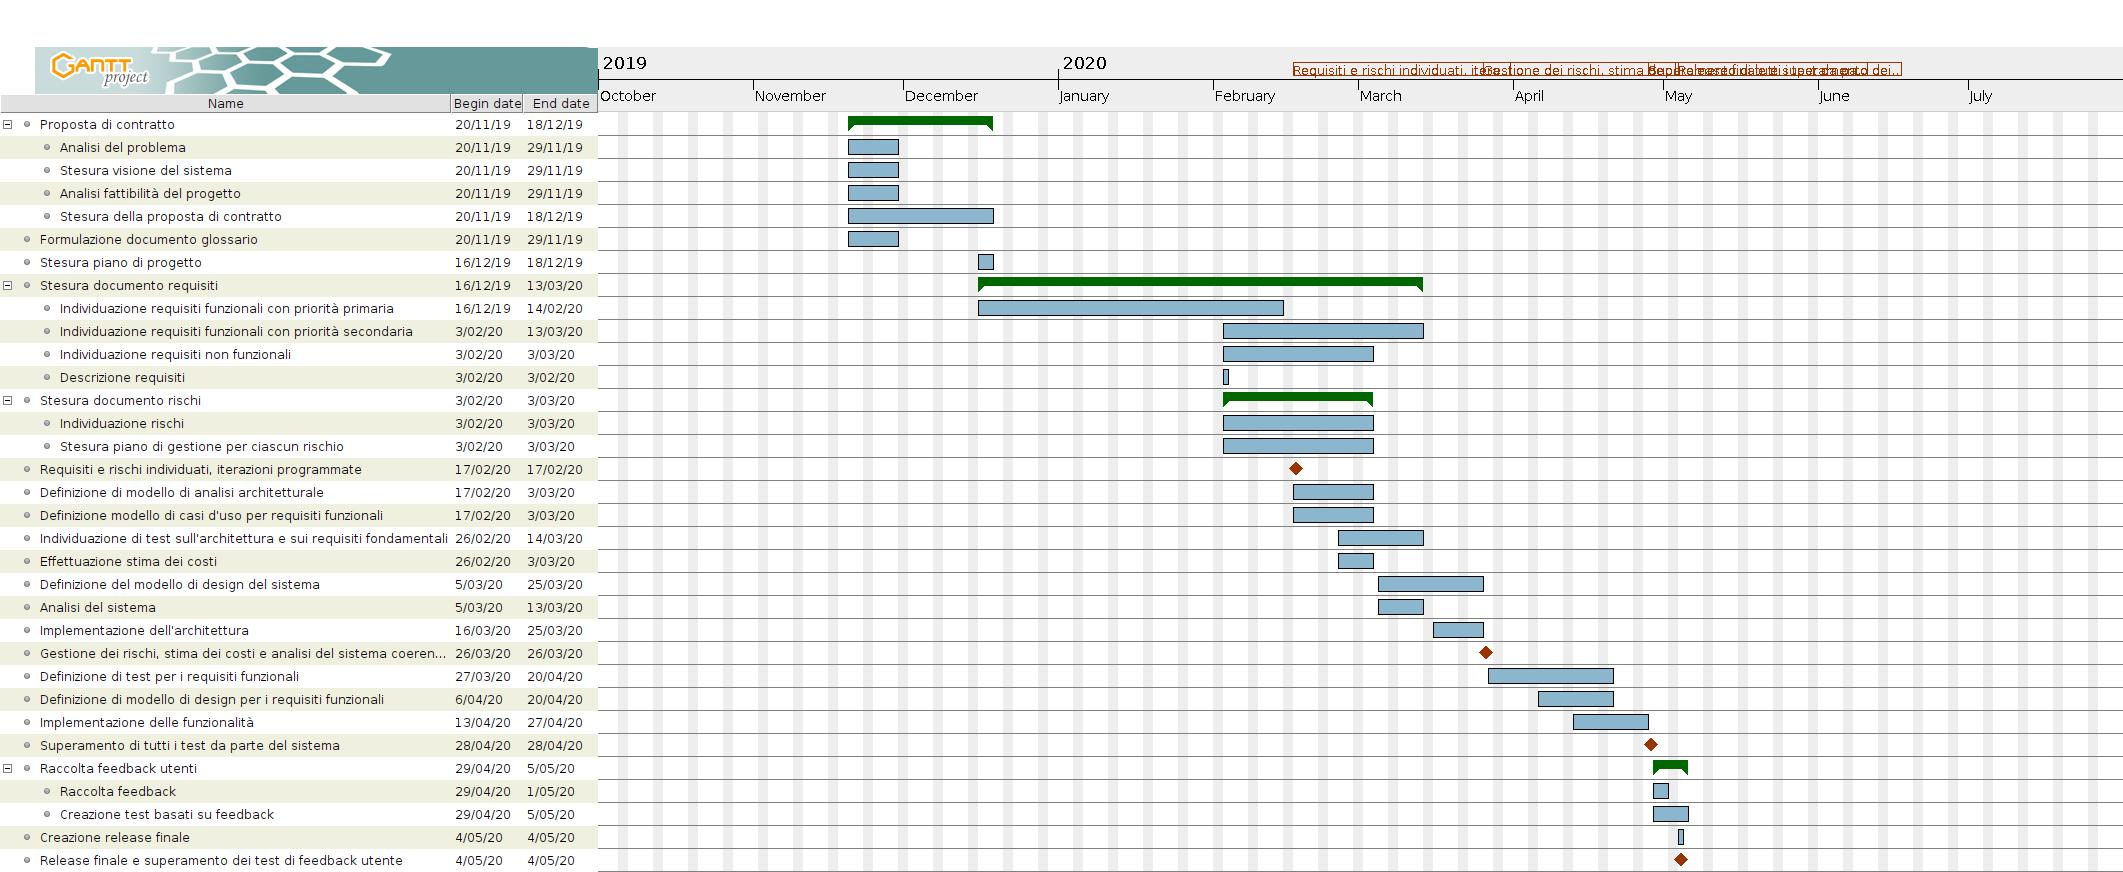
\includegraphics[width=16cm]{Gantt_NexiFy.jpg}
\end{center}
\vspace{2cm}

\clearpage
\noindent{\large \textbf{Revisioni 4-5}} \\ \\
\begin{tabular}{|c | c | c | c|} 
 	\hline
	 Numero & Data & Descrizione \\ [0.5ex] 
	\hline\hline
	1 & 17/12/2019 & Stesura iniziale \\ 
	\hline
	2 & 16/02/2020 & \thead{Specificati meglio gli obiettivi da raggiungere per ogni iterazione,\\e non gli strumenti usati per raggiungerli} \\ 
	\hline
	3 & 26/02/2020 & Revisione del contratto e del piano di progetto \\ 
	\hline
	4 & 14/03/2020 & Specificate meglio attività per implementare l'architettura\\
	\hline
\end{tabular}
\index{Index}

\newpage
\section{\itshape{Revisioni}}
\begin{tabular}{|c | c | c | c|} 
 	\hline
	 Numero & Data & Descrizione \\ [0.5ex] 
	\hline\hline
	1 & 21/11/2019 & Stesura iniziale \\ 
	\hline
	2 & 27/11/2019 & Modifica sulla gestione dei dati per analytics \\
	\hline
\end{tabular}
\index{Index}


\end{document}
